\section{Overview}

\begin{frame}
\frametitle{Today's Overview}
\begin{itemize}
	\visible<2->{\item 9:00 Intro of Deep Learning}
	\visible<3->{\item 9:30 Build and train a Perceptron in numpy}
	\visible<4->{\item 10:00 Move the code to the GPU using PyTorch}
	\visible<5->{\item 11:00 Use a neural network for more complex time-series forecasting}
	\visible<6->{\item 13:00 Introduction to NLP}
	\visible<7->{\item 15:00 TCN vs. RNN}
\end{itemize}
\end{frame}

\section{Introduction}
\begin{frame}
\frametitle{Why Deep Learning?}
\begin{itemize}
	\visible<3->{\item{It can save a lot of time of boooooring feature engineering and writing exceptions}}
	\visible<4->{\item{It can write computational rules nobody of us would ever think of}}
	\visible<5->{\item{It can often write better computational rules than we could}}
	\visible<6->{\item{It can check more cases than we could}}
\end{itemize}
\end{frame}

\begin{frame}
\frametitle{Perceptron}
\begin{figure}[h]
	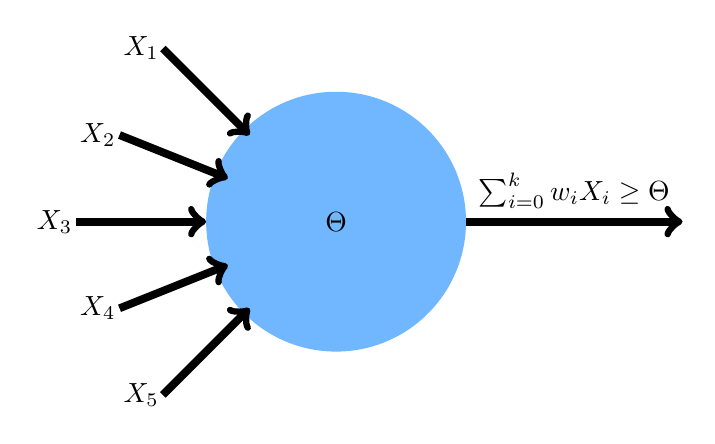
\begin{tikzpicture}[scale=.55]
		\definecolor{lightblue}{rgb}{.2,.6,1}
		\definecolor{lightred}{rgb}{.8,.2,.2}
		\definecolor{lila}{rgb}{.6,.2,.6}
		\visible<2->{\coordinate (Unit) at (0,0);
			\fill[fill=lightblue, opacity = .7] (Unit) circle(3);
			\draw (Unit) node{$\Theta$};}
		\visible<3->{
			\coordinate (x1) at (-4,4);
			\draw (x1) ++(-.5,0) node{$X_1$};
			\coordinate (x2) at (-5,2);
			\draw (x2) ++(-.5,0) node{$X_2$};
			\coordinate (x3) at (-6,0);
			\draw (x3) ++(-.5,0) node{$X_3$};
			\coordinate (x4) at (-5,-2);
			\draw (x4) ++(-.5,0) node{$X_4$};
			\coordinate (x5) at (-4,-4);
			\draw (x5) ++(-.5,0) node{$X_5$};
		}
		\visible<4->{
			\draw[->, line width=1mm] (x1) -- (-2,2);
			\draw[->, line width=1mm] (x2) -- (-2.5,1);
			\draw[->, line width=1mm] (x3) -- (-3,0);
			\draw[->, line width=1mm] (x4) -- (-2.5,-1);
			\draw[->, line width=1mm] (x5) -- (-2,-2);
		}
		\visible<5->{
			\draw[->, line width=1mm, decorate] (3,0) -- node[above]{$\sum_{i=0}^{k} w_i X_i \geq \Theta$} (8,0) ;
		}
	\end{tikzpicture}
\end{figure}
\visible<6->{A perceptron can represent every arbitary! boolean function!}
\end{frame}

\begin{frame}
\frametitle{Perceptron Training}
\begin{itemize}
	\visible<2->{\item Start with random weights}
	\visible<3->{\item{Calculate the perceptron's estimate of the solution with: $\hat{y} = \left(\sum_i w_i X_i \geq 0\right)$}}
	\visible<4->{\item{Determine the update for the weights using the error and the learning rate: $\partial w_i = \eta (y-\hat{y}) X_i$}}
	\visible<5->{\item{Calculate new weights as: $w_i = w_i + \partial w_i$}}
	\visible<6->{\item Restart the process until the solution is found}
	\visible<7->{\item Let us actually implement that in the first notebook (Perceptron)}
\end{itemize}
\end{frame}

\begin{frame}
\frametitle{Conclusions}
\begin{itemize}
	\visible<2->{\item Congratulations on training your first perceptron! You just taught a computer to learn!}
	\visible<3->{\item Why didn't we wait for the final weights?}
\end{itemize}
\end{frame}

\begin{frame}[fragile]
\frametitle{Linear Separability}
\begin{minipage}{.45\textwidth}
	\begin{tikzpicture}
	\begin{axis}[xlabel={$x$}, ylabel={$y$}, domain=0:1, width=\textwidth]
	\only<2->{
		\addplot+[scatter, only marks, scatter src=\thisrow{class},
		domain=0:1]
		table[x=x,y=y,col sep=comma,row sep=crcr] {
			x,y,class\\
			0,0,0\\
			.4,.05,0\\
			.3,.2,0\\
			.1,.1,0\\
			.2,.3,0\\
			.1,.35,0\\
			.7,.6,1\\
			.5,.5,1\\
			.4,.4,1\\
			.5,.3,1\\
			.6,.1,1\\
			.2,.6,1\\
			.8,.1,1\\
			.6,.1,1\\
			.2,.6,1\\
	};}
	\only<3->{\addplot+[no marks, domain=0:.6] {-x+.6};}
	\end{axis}
	\end{tikzpicture}
	
\end{minipage}
\hfill
\begin{minipage}{.45\textwidth}
	\only<4->{
	\begin{tikzpicture}
	\begin{axis}[xlabel={$x$}, ylabel={$y$},domain=0:1, width=\textwidth]
		\addplot+[scatter, only marks, scatter src=\thisrow{class},
		domain=0:1]
		table[x=x,y=y,col sep=comma,row sep=crcr] {
			x,y,class\\
			0,0,0\\
			.4,.05,0\\
			.6,.5,0\\
			.1,.35,0\\
			.2,.3,0\\
			.1,.35,0\\
			.7,.6,1\\
			.3,.2,1\\
			.4,.4,1\\
			.5,.3,1\\
			.6,.1,1\\
			.2,.6,1\\
			.8,.1,1\\
			.6,.1,1\\
			.2,.6,1\\
		};
	\end{axis}
	\end{tikzpicture}
	}

\end{minipage}
\visible<5->{The algorithm only converges, if the problem is linearly separable.}

\end{frame}

\begin{frame}
\frametitle{Gradient Descent}
\begin{itemize}
	
	\begin{minipage}{.45\textwidth}
		\visible<2->{\item What we calculated is an activation $a=\sum_i w_i X_i$}
		\visible<3->{\item Let us ignore the threshold and try to get the activation as close to the target value as possible. }
		\visible<4->{\item This brings us back to regression with an error: $E(w) = \frac12 \sum_{(x,y) \in D} (y-a)^2$ }
		\visible<6->{\item If we want to decrease $E(w)$ by changing $w$ we need to calculate the gradient of $w$}
		\visible<7->{\item Every deep learning framework can calculate those weights using the chain rule and backpropagation.}
	\end{minipage}
	\hfill
	\begin{minipage}{.45\textwidth}
		\only<4->{\begin{tikzpicture}
		\begin{axis}[xlabel={$x$}, ylabel={$y$}, domain=0:1, width=\textwidth]
		\only<4->{\addplot+[no marks, domain=-1:1] {x*x};}
		\only<5->{
			\addplot+[scatter, only marks, scatter src=\thisrow{class},
			domain=0:1]
			table[x=x,y=y,col sep=comma,row sep=crcr] {
				x,y,class\\
				0,0,1\\
				.9,.81,0\\
			};}
		\only<6->{
			\node[anchor=west] (source) at (axis cs:.85,.85){};
			\node (destination) at (axis cs:.5,.1){};
			\draw[->](source)--(destination);
		}
		\end{axis}
		\end{tikzpicture}}
		
	\end{minipage}
\end{itemize}
\end{frame}

\begin{frame}
\frametitle{Sigmoid $\rightarrow$ Differentiable Threshold}
\begin{minipage}{.45\textwidth}
\begin{itemize}
	\visible<2->{\item Even though the perceptron is great for boolean functions it is not differentiable and has no continuous error function}
	\visible<3->{\item $\sigma(a) = \frac{1}{1+e^{-a}}$}
	\visible<4->{\item The sigmoid allows us to convert the strict classification into a regression over the probability to classify the points}
\end{itemize}
\end{minipage}
\hfill
\begin{minipage}{.45\textwidth}
\visible<3->{\begin{tikzpicture}
	\draw[->] (-2.5,0) -- (2.5,0);
	\draw[->] (-2.5,0) -- (-2.5,3);
	\node at (-2.7,0) {0};
	\node at (-2.7,3) {1};
	\node at (-1.666,-.2) {-5};
	\node at (0,-.2) {0};
	\node at (1.6666,-.2) {5};
	\draw[scale=1,domain=-2.5:2.5,smooth,variable=\x,blue] plot ({\x},{3/(1+exp(-3*\x)))});
	\end{tikzpicture}}
\end{minipage}
\end{frame}

%\begin{frame}
%\frametitle{Backpropagation}
%\begin{minipage}{.59\textwidth}
%	\begin{itemize}
%	\visible<2->{\item How do we do gradient descent now?}
%	\visible<3->{\item Activation: $a = W^{(1)} \circ x$}
%	\visible<4->{\item Prediction: $o = \sigma(a)$}
%	\visible<5->{\item Error Function $E(o)=-t\log o - (1-t)\log(1-o)$}
%	\visible<6->{\item Gradient: $\frac{\partial E}{\partial W} = E(o)\frac{\partial E}{\partial o}\frac{\partial o}{\partial a}\frac{\partial a}{\partial W^{(1)}}$}
%	\visible<7->{\item This allows a framework to compute gradients for every node, given that the gradient for each step is known.}
%	\end{itemize}
%\end{minipage}
%\hfill
%\begin{minipage}{.4\textwidth}
%
%\begin{tikzpicture}
%\visible<3->{\foreach \i in {1,...,5} {\draw[green] (0,\i) -- (1.5,3);}}
%\visible<4->{\draw[green] (1.5,3) -- (3,3);}
%\visible<5->{\draw[green] (3,3) -- (4.5,3);}
%\visible<2->{\foreach \y in {1,...,5} \draw(0,\y) node[left, circle, draw=black]{$X_\y$};}
%\visible<3->{\draw(1.5, 3) node[circle, draw=black, fill=white]{$W^{(1)}$};}
%\visible<4->{\draw(3, 3) node[circle, draw=black, fill=white]{$\sigma$};}
%\visible<5->{\draw(4.5, 3) node[circle, draw=black, fill=white]{BCE};}
%\end{tikzpicture}
%\end{minipage}
%	
%
%\end{frame}

%\begin{frame}
%\frametitle{Comparison of the learning rules}
%\begin{itemize}
%	\visible<2->{\item{Perceptron Rule: $w_i = w_i + \eta (y-\hat{y}) X_i$
%		\begin{itemize}
%			\item Guaranteed to converge, if problem is seperable
%			\item Finite number of steps
%		\end{itemize}
%	}}
%	\visible<3->{\item{Gradient Descent: $w_i = w_i + \eta(y-a) X_i$
%		\begin{itemize}
%			\item Robust due to the continuously differentiable functions
%			\item Only converges in the limit and only to local optima
%		\end{itemize}
%	}}
%\end{itemize}
%\end{frame}

%\begin{frame}
%\frametitle{Numerical Instability}
%\begin{minipage}{.45\textwidth}
%	\begin{itemize}
%		\visible<2->{\item The derivative of sigma is $\frac{\partial\sigma(a)}{\partial a} = \sigma(a)(1-\sigma(a))$}
%		\visible<3->{\item Derivative for t=0: $-\frac{1}{\sigma{(a)}} * err$}
%		\visible<4->{\item Derivative for t=1: $-\frac{1}{1- \sigma{(a)}} * err$}
%		\visible<5->{\item t=0, $\sigma{(a)}$=0: $err = 0$, $\sigma{(a)}=1$: $err = \infty$}
%		\visible<6->{\item t=1, $\sigma{(a)}=0$: $err = \infty$, $\sigma{(a)}=1$: $err = 0$}
%	\end{itemize}
%\end{minipage}
%\hfill
%\begin{minipage}{.45\textwidth}
%	\visible<4->{\begin{tikzpicture}
%		\draw[->] (-2.5,0) -- (2.5,0);
%		\draw[->] (-2.5,0) -- (-2.5,3);
%		\node at (-2.7,0) {0};
%		\node at (-2.7,3) {1};
%		\node at (-1.666,-.2) {-5};
%		\node at (0,-.2) {0};
%		\node at (1.6666,-.2) {5};
%		\draw[scale=1,domain=-2.5:2.5,smooth,variable=\x,blue] plot ({\x},{3/(1+exp(-3*\x)) * (3-3/(1+exp(-3*\x))});
%		\draw[scale=1,domain=.2:1,smooth,variable=\x,orange] plot ({\x},{-(1+exp(-\x))});
%		\draw[scale=1,domain=.2:1,smooth,variable=\x,orange] plot ({\x},{1/(1-1/(1+exp(-\x)))});
%		\end{tikzpicture}}
%\end{minipage}
%\end{frame}


\begin{frame}
\frametitle{Softmax}
\begin{itemize}
	\visible<2->{\item To generalize to n-classification problems we have to extend the function, that calculates the probability}
	\visible<3->{\item Softmax: $p = \frac{e^{o_i}}{\sum_i{e^{o_i}}}$}
	\visible<4->{\item With this we can as well define the general loss}
	\visible<5->{\item Cross- Entropy $E=-\frac1n\sum_{i=1}^n\sum_{k=1}^m{y_{i,k}\ln{p_{i,k}}}$}
\end{itemize}
\end{frame}

\begin{frame}
\frametitle{Neural Network}
\begin{minipage}{.45\textwidth}
\begin{itemize}
	\visible<2->{\item Similar to the perceptron we have a lot of inputs and an output}
	\visible<3->{\item However, instead of going from start to end directly we now add hidden units}
	\visible<4->{\item For each of the units we now apply the sigmoid function}
	\visible<5->{\item Since every unit is differentiable, the whole network is differentiable $\rightarrow$ We can use backpropagation to minimise the error as we can calculate the gradients}
\end{itemize}
\end{minipage}
\hfill
\begin{minipage}{.54\textwidth}

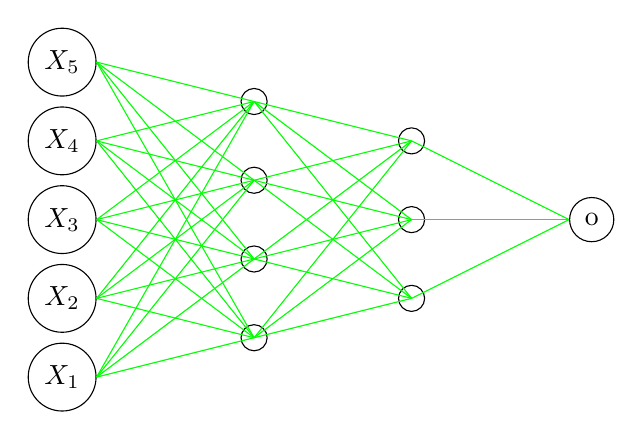
\begin{tikzpicture}
	\visible<2->{\foreach \y in {1,...,5} \draw(0,\y) node[left, circle, draw=black]{$X_\y$};
		\draw(6, 3) node[right, circle, draw=black]{o};}

	\visible<3->{\foreach \y in {1,...,4} \draw(2,\y+.5) node[circle, draw=black]{};
		\foreach \y in {2,...,4} \draw(4,\y) node[circle, draw=black]{};}
	\visible<4->{\foreach \y in {1,...,4} \foreach \i in {1,...,5} {\draw[green] (0,\i) -- (2,\y+.5);}
		\foreach \y in {2,...,4} \foreach \i in {1.5,...,4.5} {\draw[green] (2,\i) -- (4,\y);}
		\foreach \i in {2,...,4} {\draw[green] (4,\i) -- (6,3);}
	}
\end{tikzpicture}
\end{minipage}
\end{frame}



\begin{frame}
\frametitle{Optimising Weights}
\begin{itemize}
	\visible<2->{\item Gradient Descent}
	\visible<3->{\item Advanced Methods
		\begin{itemize}
			\visible<4->{\item Momentum}
			\visible<5->{\item Higher Order Derivatives}
			\visible<6->{\item Randomised Optimisation}
			\visible<7->{\item Penalty for Complexity}
		\end{itemize}

	}
\end{itemize}

\end{frame}

\begin{frame}
\frametitle{Restriction Bias}
\begin{itemize}
	\visible<2->{\item Representational power of the algorithm due to the hypothesis considered}
	\visible<3->{\item Perceptron $\rightarrow$ half spaces}
	\visible<4->{\item Sigmoids $\rightarrow$ non-linear function}
	\visible<5->{\item What can we represent with a network?
		\begin{itemize}
			\visible<6->{\item Boolean Functions: Yes, because we have a network of threshold-like units}
			\visible<7->{\item Continous Functions: Yes, with one (infinitly wide) hidden layer}
			\visible<8->{\item Arbitrary Functions: Yes, with two (infinitly wide) hidden layers}
		\end{itemize}

	}
\end{itemize}

\end{frame}

\section{Frameworks}
\begin{frame}
\frametitle{Available Deep Learning Frameworks}
\begin{itemize}
	\visible<2->{\item \href{http://tensorflow.org}{TensorFlow}}
	\visible<3->{\item \href{http://caffe2.ai}{Caffe}}
	\visible<4->{\item \href{http://pytorch.org}{PyTorch}}
	\visible<5->{\item Theano (Deprecated)}
	\visible<6->{\item \href{http://keras.io}{Keras}}
\end{itemize}

\end{frame}

\begin{frame}
\frametitle{Advantages, Disadvantages}
	\begin{table}[h]
		\begin{tabular}{|c|c|c|}
		\hline
		Framework & Advantages & Disadvantages \\
		\hline
		\visible<2->{TensorFlow} &
		\visible<3->{\begin{tabular}{c}Huge Community  \\ Easy Conversion for mobile devices\end{tabular}} &
		\visible<4->{\begin{tabular}{c}Graphs are relatively static \\ No real integration into Python\end{tabular}}\\
		\hline
		\visible<5->{PyTorch} &
		\visible<6->{\begin{tabular}{c}Perfect integration into Python Objects \\ Graph can be dynamically changed without rebuilding it \\ Will probably be integrated into TensorRT \end{tabular}} &
		\visible<7->{Still quite new}\\
		\hline
		\visible<8->{Caffe} &
		\visible<9->{\begin{tabular}{c} Big Community \\ Very well integrated into TensorRT A bit more\end{tabular}} &
		\visible<10->{\begin{tabular}{c}Graphs are relatively static \\ No real integration into Python\end{tabular}}\\
		\hline
		\end{tabular}
	\end{table}
\end{frame}

\begin{frame}
\frametitle{Tensorflow Tutorials}
\begin{itemize}
	\visible<2->{\item Let us have a look at some TensorFlow examples}
	\visible<3->{\item Use the terminal to navigate to TensorFlow-Examples/notebooks and run 'jupyter notebook'}
\end{itemize}

\end{frame}

\begin{frame}
\frametitle{Small Test: Traffic Sign Classifier}
\begin{itemize}
	\visible<2->{\item Let's see what you learned.}
	\visible<3->{\item Use the terminal to navigate to TrafficSignClassifier and run 'jupyter notebook'}
	\visible<4->{\item Try solving the given problem with a network of your choice}
\end{itemize}

\end{frame}

\section{SegNet}
\begin{frame}
\frametitle{Motivation}
\begin{minipage}{.45\textwidth}
\begin{itemize}
	\visible<2->{\item Just assigning an image to class is not sufficent in lots of situations}
	\visible<3->{What label would you assign?
		\begin{itemize}
			\visible<4->{\item Image from Car?}
			\visible<5->{\item Street?}
			\visible<5->{\item Traffic Lights?}
			\visible<6->{\item Akka Hamburg?}
		\end{itemize}
		}
	\visible<7->{\item We clearly need another approach, if we want to have a car driving}
\end{itemize}
\end{minipage}
\hfill
\begin{minipage}{.45\textwidth}
	\visible<3->{
		\includegraphics[width=\textwidth]{./figs/hamburg_000000_013577_leftImg8bit.png}}
\end{minipage}
\end{frame}

\begin{frame}
\frametitle{Bounding Boxes}
\begin{minipage}{.45\textwidth}
\visible<1->{
		\includegraphics[width=\textwidth]{./figs/hamburg_000000_013577_leftImg8bit.png}}
\end{minipage}
\hfill
\begin{minipage}{.45\textwidth}
	\visible<2->{
		\includegraphics[width=\textwidth]{./figs/hamburg_000000_013577_leftImg8bitAnno.png}}
\end{minipage}
\end{frame}

\begin{frame}
\frametitle{Semantic Segmentation}
\begin{minipage}{.45\textwidth}
\visible<1->{
		\includegraphics[width=\textwidth]{./figs/hamburg_000000_013577_leftImg8bit.png}}
\end{minipage}
\hfill
\begin{minipage}{.45\textwidth}
	\visible<2->{
		\includegraphics[width=\textwidth]{./figs/hamburg_000000_013577_gtFine_color.png}}
\end{minipage}
\end{frame}

\begin{frame}
\frametitle{Network Structure}
\includegraphics[width=\textwidth]{./figs/segNetStructure.png}
\end{frame}

\begin{frame}
\frametitle{Implementation}
\begin{itemize}
	\visible<1->{\item Let's investigate how to programm a SegNet}
	\visible<2->{\item Use the terminal to navigate to SegNet and run 'jupyter notebook'}
	\visible<3->{\item We probably cannot run it as it takes 6+ GB of VRAM}
\end{itemize}

\end{frame}
